% GraphQL-Shield -- Review 3 presentation (Beamer)
% Compile: pdflatex slides.tex  (run twice)   -- figures are in ./figures
\documentclass[aspectratio=169,11pt]{beamer}
\usetheme{Madrid}
\usepackage[utf8]{inputenc}
\usepackage[T1]{fontenc}
\usepackage{lmodern}
\usepackage{booktabs,array,colortbl}
\usepackage[most]{tcolorbox}
\graphicspath{{figures/}}

\definecolor{navy}{HTML}{1F3A5F}
\definecolor{teal}{HTML}{1690A8}
\definecolor{tealbg}{HTML}{E6F4F7}
\definecolor{rowgrey}{HTML}{F2F4F7}
\setbeamercolor{structure}{fg=navy}
\setbeamercolor{palette primary}{bg=navy,fg=white}
\setbeamercolor{palette secondary}{bg=teal,fg=white}
\setbeamercolor{palette tertiary}{bg=navy,fg=white}
\setbeamercolor{frametitle}{bg=navy,fg=white}
\setbeamercolor{title}{bg=navy,fg=white}
\setbeamercolor{block title}{bg=teal,fg=white}
\setbeamertemplate{navigation symbols}{}
\setbeamertemplate{itemize item}{\color{teal}$\blacktriangleright$}
\setbeamertemplate{itemize subitem}{\color{teal}--}
\setbeamerfont{itemize/enumerate subbody}{size=\small}

% "In simple words" box for non-technical listeners
\newtcolorbox{simplebox}{enhanced,colback=tealbg,colframe=teal,boxrule=0.6pt,arc=2pt,
  left=6pt,right=6pt,top=3pt,bottom=3pt,fontupper=\small,
  title={\small\textbf{In simple words}},coltitle=white,colbacktitle=teal,
  attach boxed title to top left={xshift=6pt,yshift*=-\tcboxedtitleheight/2},top=7pt,boxed title style={boxrule=0pt,arc=2pt}}

\title[GraphQL-Shield]{GraphQL-Shield}
\subtitle{Dual-Layer Protection of GraphQL APIs against Broken Object Level Authorization (BOLA)}
\author[Team Name]{[Student Name 1] \and [Student Name 2] \and [Student Name 3] \and [Student Name 4]}
\institute[]{Guide: [Guide Name], [Designation]\\[2pt] Department of [Department], [College / University Name]}
\date{Review 3}

\begin{document}

\begin{frame}
  \titlepage
\end{frame}

\begin{frame}{Outline}
  \begin{columns}[T]
    \begin{column}{0.48\textwidth}
      \begin{enumerate}
        \item Introduction
        \item Problem Statement \& Motivation
        \item Objectives
        \item Literature Survey
        \item Research Gap
        \item Proposed System
        \item System Architecture / Methodology
      \end{enumerate}
    \end{column}
    \begin{column}{0.48\textwidth}
      \begin{enumerate}\setcounter{enumi}{7}
        \item Implementation
        \item Results and Discussion
        \item Conclusion
        \item Future Scope
        \item References
        \item Research Paper Template
      \end{enumerate}
    \end{column}
  \end{columns}
\end{frame}

%% ============================================================
\section{Introduction}
\begin{frame}{What is an API, and what is GraphQL?}
\begin{itemize}
\item Apps (Instagram, banking, hospital portals) talk to their servers through an \textbf{API}.
\item \textbf{GraphQL} is a modern API style made by Facebook: one address, and the app asks for \emph{exactly} the data it wants.
\begin{itemize}
\item Example: “give me my name, my documents, and the files inside my folder” – in one request.
\end{itemize}
\item Flexible and fast – so it is now widely used.
\item But the flexibility opens a new security hole.
\end{itemize}
\vfill
\begin{simplebox}REST is like a fixed restaurant menu. GraphQL is like telling the waiter exactly what to bring. Very convenient – but the kitchen must still check that you only get \emph{your} order.\end{simplebox}
\end{frame}
\begin{frame}{The Threat: BOLA}
\begin{itemize}
\item \textbf{BOLA = Broken Object Level Authorization.}
\item The server knows \emph{who} you are (you logged in), but forgets to check whether the item you asked for is \emph{yours}.
\item Attacker simply changes a number: \texttt{resource(id: 101)} $\rightarrow$ \texttt{resource(id: 102)} and reads someone else’s data.
\item Ranked \textbf{\#1 risk} in the OWASP API Security Top 10 (2023).
\item Firewalls cannot see it – the request looks completely normal.
\end{itemize}
\vfill
\begin{simplebox}Like a hotel key card that opens every room if you just type a different room number. You are a real guest – but you should only open your own room.\end{simplebox}
\end{frame}
\begin{frame}{Our Solution in One Line}
\begin{itemize}
\item \textbf{GraphQL-Shield}: a security gateway placed in front of any GraphQL app.
\item It checks ownership at \textbf{two independent points}:
\begin{itemize}
\item \textbf{Layer 1} – before the request runs: “does this request name anything that isn’t yours?”
\item \textbf{Layer 2} – while it runs: “is every item actually being returned or changed yours?”
\end{itemize}
\item Novel idea: Layer 2 also \textbf{reports what Layer 1 missed}, so the system measures and repairs its own gaps.
\end{itemize}
\vfill
\begin{simplebox}Two security guards: one at the hotel entrance checks your request, one in the corridor checks every door you open – and writes down anything the entrance guard missed.\end{simplebox}
\end{frame}

%% ============================================================
\section{Problem Statement \& Motivation}
\begin{frame}{Problem Statement}
\begin{itemize}
\item \textbf{Problem:} Design and implement a runtime defence that stops logged-in users of a GraphQL API from reading or changing objects they do not own – in every form GraphQL allows – while:
\begin{itemize}
\item keeping legitimate access working,
\item adding very little delay,
\item and showing where the defence itself is incomplete.
\end{itemize}
\end{itemize}
\begin{center}
\small
\renewcommand{\arraystretch}{1.12}
\begin{tabular}{>{\raggedright\arraybackslash}p{0.205\linewidth}>{\raggedright\arraybackslash}p{0.410\linewidth}>{\raggedright\arraybackslash}p{0.246\linewidth}}
\toprule
\textbf{Form of attack} & \textbf{Example} & \textbf{ID visible in request?} \\
\midrule
Direct & resource(id: 102) & Yes \\
\rowcolor{rowgrey}Nested & user(id:101)\{resource(id:102)\} & Yes, deeper \\
Disguised & variable, alias, fragment, batch & Only after decoding \\
\rowcolor{rowgrey}Relationship & folder(201)\{children\{...\}\} & No – hidden \\
Write & updateResource(id:102, ...) & Yes \\
\bottomrule
\end{tabular}
\end{center}
\end{frame}
\begin{frame}{Motivation – Why This Matters}
\begin{itemize}
\item BOLA directly causes data breaches of personal, medical and financial records.
\item Existing tools only \textbf{test} for BOLA before release, or need a hand-written rule for \textbf{every field} – one forgotten rule silently leaks data.
\item Checking only the request cannot see items reached through links (folder $\rightarrow$ children).
\item Wrongly placed blocks in GraphQL can wipe out the user’s \textbf{own} data too (null propagation).
\item No existing defence tells the developer \textbf{where it is weak}.
\end{itemize}
\vfill
\begin{simplebox}Current locks either get checked once at the factory, or need a separate lock on every drawer. We want a lock that checks itself and tells you when a drawer was left open.\end{simplebox}
\end{frame}

%% ============================================================
\section{Objectives}
\begin{frame}{Objectives}
\begin{itemize}
\item \textbf{Block every form of BOLA} – direct, nested, disguised, relationship and write attacks.
\item \textbf{Defence in depth:} two independent layers (before and during execution).
\item \textbf{Cross-layer evidence:} Layer 2 records every object Layer 1 never checked.
\item \textbf{Blind-spot prediction:} XGBoost model with SHAP explanations, trained from that evidence.
\item \textbf{Self-repairing configuration:} verified fixes, applied only with admin approval.
\item \textbf{Formal security properties} (Safety, Non-interference, Write safety, Availability) tested automatically.
\item \textbf{Close side channels} – same error and same timing for “not yours” and “does not exist”.
\item \textbf{Secure accounts} (hashed passwords, lockout, token revocation) and \textbf{low overhead} (\textasciitilde{}1 ms).
\end{itemize}
\end{frame}

%% ============================================================
\section{Literature Survey}
\begin{frame}{Literature Survey}
\begin{center}
\footnotesize
\renewcommand{\arraystretch}{1.05}
\begin{tabular}{>{\raggedright\arraybackslash}p{0.287\linewidth}>{\raggedright\arraybackslash}p{0.323\linewidth}>{\raggedright\arraybackslash}p{0.251\linewidth}}
\toprule
\textbf{Work} & \textbf{Approach} & \textbf{Limitation for us} \\
\midrule
OWASP API Top 10 (2023) [1] & Ranks BOLA as \#1 API risk & Guidance only \\
\rowcolor{rowgrey}GraphQLer (Tsai et al., 2025) [2] & Replays GraphQL requests as other users & Test-time, no runtime blocking \\
AuthProbe (Barach, 2026) [3] & Multi-identity BOLA testing from OpenAPI & REST only, test-time \\
\rowcolor{rowgrey}Santos Filho et al. (2025) [4] & OpenAPI $\rightarrow$ Petri nets attack models & REST only, detection \\
BolaZ (Wu et al., 2026) [5] & Static taint + runtime checks (Spring Boot) & Java REST, no self-measurement \\
\rowcolor{rowgrey}Lambers et al. (2026) [6] & Taint analysis for graph APIs & Static only \\
graphql-shield library [7] & Permission rule per type/field & Many rules; can null own data \\
\rowcolor{rowgrey}Hartig \& Pérez; Cha et al. [8],[9] & GraphQL semantics, query cost & Not about ownership \\
Kaur (2026) [11]; CVE-2022-39275 [12] & 100+ real BOLA bug reports; Saleor ID bug & Shows the threat is real \\
\bottomrule
\end{tabular}
\end{center}
\end{frame}
\begin{frame}{Key Observations from the Survey}
\begin{itemize}
\item \textbf{Testing tools} find BOLA before deployment but give no protection at runtime – and most target REST, not GraphQL.
\item \textbf{Enforcement tools} either inspect only the request (miss relationship links) or need one rule per field (leak when one is forgotten).
\item \textbf{GraphQL research} studies query cost and semantics, not \emph{who owns} the data.
\item \textbf{Classic security principles} – reference monitor, complete mediation, non-interference – are well known but never combined into a self-checking GraphQL defence.
\end{itemize}
\vfill
\begin{simplebox}Others built either a scanner (finds problems before opening day) or a rulebook (one rule per door). Nobody built a guard that also audits itself.\end{simplebox}
\end{frame}

%% ============================================================
\section{Research Gap}
\begin{frame}{Research Gap}
\begin{itemize}
\item \textbf{1.} No runtime defence covers \textbf{all} GraphQL BOLA forms (relationship links are missed).
\item \textbf{2.} No defence \textbf{measures itself} – none uses one layer to check another’s coverage.
\item \textbf{3.} No \textbf{automatic, verified repair} of a wrong security configuration.
\item \textbf{4.} \textbf{Availability ignored} – rule-based tools can delete the user’s own data from the answer.
\item \textbf{5.} \textbf{Side channels} – different errors or timings reveal which objects exist.
\item \textbf{6.} No stated and \textbf{tested security properties}.
\item \textbf{7.} Tied to \textbf{one framework}.
\end{itemize}
\vfill
\begin{simplebox}GraphQL-Shield is designed to close each of these seven gaps.\end{simplebox}
\end{frame}

%% ============================================================
\section{Proposed System}
\begin{frame}{Proposed System: GraphQL-Shield}
\begin{itemize}
\item Configured once with a small \textbf{ShieldConfig}: which data types are private, and how to find an item’s owner.
\item \textbf{No security code needed inside the app} itself.
\item \textbf{Attacker model:} a real, logged-in user who tries to read or change other people’s items.
\item \textbf{Four guarantees} (for a normal user \emph{u}):
\begin{itemize}
\item \textbf{P1 Safety} – the answer never contains another user’s object.
\item \textbf{P2 Non-interference} – changing other users’ data never changes \emph{u}’s answer.
\item \textbf{P3 Write safety} – \emph{u} can never modify or delete others’ objects.
\item \textbf{P4 Availability} – \emph{u}’s own objects are always returned.
\end{itemize}
\end{itemize}
\end{frame}
\begin{frame}{Main Components}
\begin{itemize}
\item \textbf{Layer 1 – Entrance gate:} reads the request before it runs; any foreign ID $\rightarrow$ HTTP 403, nothing executes.
\item \textbf{Layer 2 – Inside guard:} checks every object actually returned and every write target; removes foreign items.
\item \textbf{Cross-layer evidence:} logs every object Layer 1 never saw $\rightarrow$ shows Layer 1’s blind spots.
\item \textbf{Blind-spot predictor:} XGBoost on 17 request features (advisory only).
\item \textbf{Self-repair:} diagnoses the gap, proposes a fix, replays old traffic to verify it, admin approves.
\item \textbf{Uniform denials}, \textbf{account protection}, \textbf{tamper-evident (hash-chained) audit log}, \textbf{live dashboard}.
\end{itemize}
\end{frame}

%% ============================================================
\section{System Architecture / Methodology}
\begin{frame}{System Architecture}
\begin{center}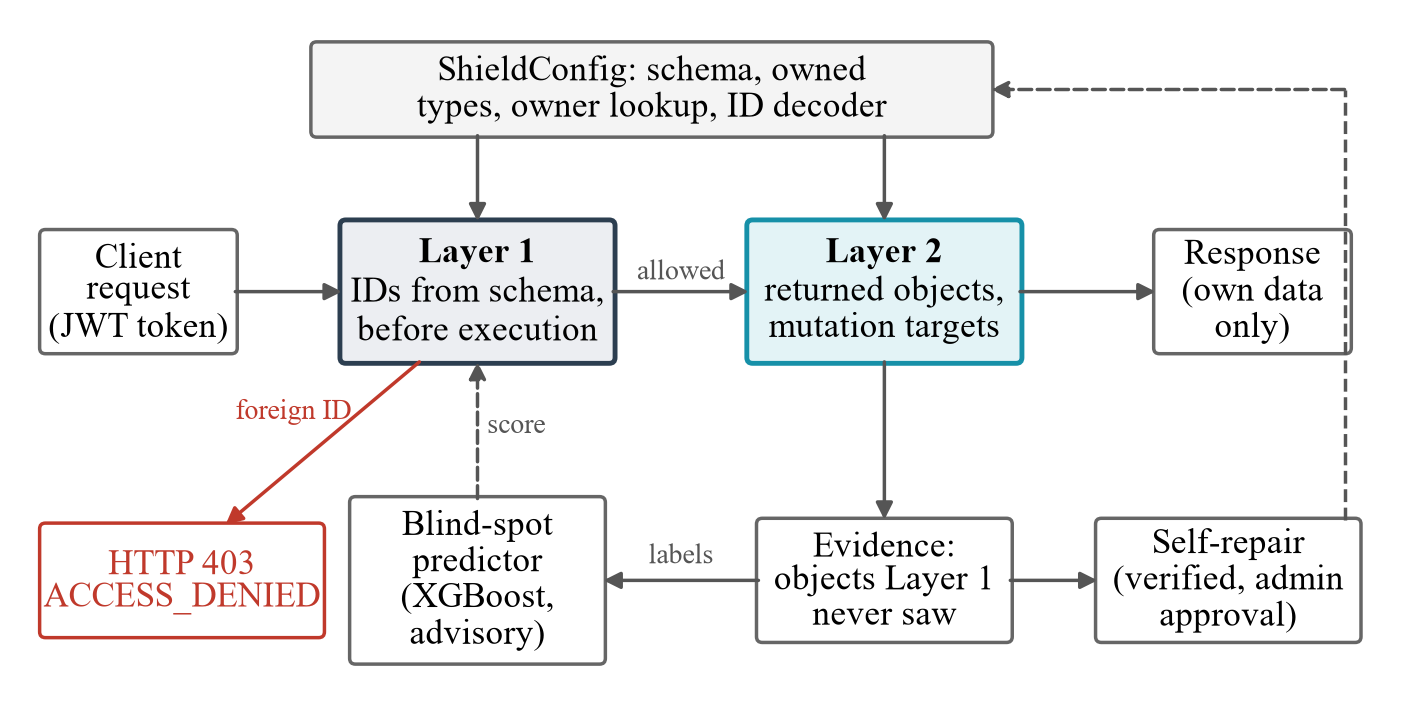
\includegraphics[width=0.92\linewidth,height=0.55\textheight,keepaspectratio]{fig7_1.png}\end{center}
\vfill
\begin{simplebox}Request $\rightarrow$ Layer 1 (block if foreign ID) $\rightarrow$ app runs $\rightarrow$ Layer 2 (remove foreign items) $\rightarrow$ only your data comes back. Disagreements between the layers feed the predictor and the self-repair module.\end{simplebox}
\end{frame}
\begin{frame}{Methodology: Life of One Request}
\begin{center}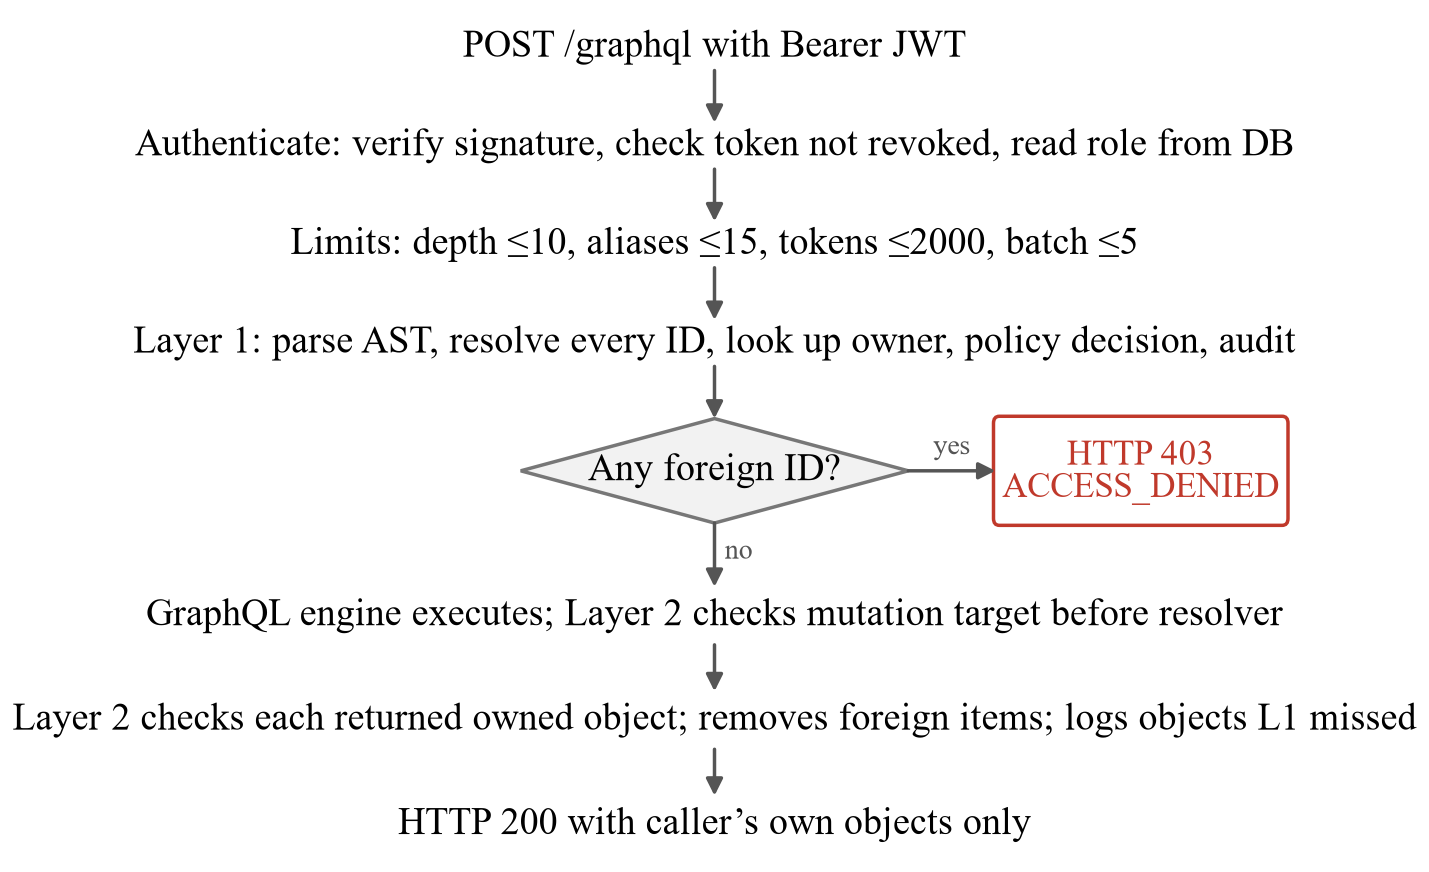
\includegraphics[width=0.78\linewidth,height=0.80\textheight,keepaspectratio]{fig7_2.png}\end{center}
\end{frame}
\begin{frame}{Methodology: How Each Part Works}
\begin{itemize}
\item \textbf{Layer 1:} walks the parsed query, decodes every ID (variables, defaults, aliases, fragments, batches, Relay IDs), looks up the owner – one foreign ID rejects the whole request.
\item \textbf{Layer 2:} runs inside the GraphQL engine; checks the real mutation target before the write; filters lists \emph{before} GraphQL’s null rules apply, so your own data survives.
\item \textbf{Evidence:} Layer 1 marks what it checked; Layer 2 records anything unmarked = proof of a Layer 1 gap.
\item \textbf{Self-repair:} a fix is offered only if replay shows it closes gaps and blocks no legitimate request.
\item \textbf{Evaluation:} 6 research questions – ablation, fault detection, properties, comparison, latency, self-repair.
\end{itemize}
\end{frame}

%% ============================================================
\section{Implementation}
\begin{frame}{Implementation: Technology Stack}
\begin{center}
\small
\renewcommand{\arraystretch}{1.12}
\begin{tabular}{>{\raggedright\arraybackslash}p{0.299\linewidth}>{\raggedright\arraybackslash}p{0.599\linewidth}}
\toprule
\textbf{Component} & \textbf{Technology} \\
\midrule
Language / web & Python 3.13, FastAPI, Uvicorn \\
\rowcolor{rowgrey}GraphQL & Strawberry, graphql-core, Graphene, Ariadne \\
Authentication & JWT (HS256), PBKDF2-SHA256 passwords, lockout \\
\rowcolor{rowgrey}Database & SQLite with connection pooling \\
Machine learning & XGBoost, scikit-learn, SHAP \\
\rowcolor{rowgrey}Testing & pytest, Hypothesis – 427 automated tests \\
Comparison baseline & Node.js + graphql-shield 7.6.5 \\
\rowcolor{rowgrey}Front-end / DevOps & HTML/JS dashboard, Docker, GitHub Actions \\
\bottomrule
\end{tabular}
\end{center}
\vfill
\begin{simplebox}Two separate apps are protected (a document app and a clinic app with patient records) – the clinic app has zero security code of its own.\end{simplebox}
\end{frame}
\begin{frame}{Implementation: Live Demo Scenarios}
\begin{center}
\small
\renewcommand{\arraystretch}{1.12}
\begin{tabular}{>{\raggedright\arraybackslash}p{0.244\linewidth}>{\raggedright\arraybackslash}p{0.356\linewidth}>{\raggedright\arraybackslash}p{0.262\linewidth}}
\toprule
\textbf{Demo (user 101 attacks)} & \textbf{Request} & \textbf{Outcome} \\
\midrule
Legitimate access & resource(id: 101) & 200 OK \\
\rowcolor{rowgrey}Direct BOLA & resource(id: 102) & 403 – Layer 1 \\
Nested BOLA & user(101)\{resource(102)\} & 403 – Layer 1 \\
\rowcolor{rowgrey}Unauthorised write & updateResource(102, "Hacked") & Blocked, DB unchanged \\
Relationship traversal & resource(201)\{children\} & 200 – foreign child removed \\
\rowcolor{rowgrey}Admin override & admin reads resource(102) & 200 – logged \\
\bottomrule
\end{tabular}
\end{center}
\vfill
\begin{simplebox}Dashboard (/dashboard): run every attack with one click, switch layers off to see what each one stops, view the ML models, self-repair and the audit log.\end{simplebox}
\end{frame}

%% ============================================================
\section{Results and Discussion}
\begin{frame}{Result 1: Which Layer Stops Each Attack?}
\begin{center}
\small
\renewcommand{\arraystretch}{1.12}
\begin{tabular}{>{\raggedright\arraybackslash}p{0.228\linewidth}>{\raggedright\arraybackslash}p{0.140\linewidth}>{\raggedright\arraybackslash}p{0.140\linewidth}>{\raggedright\arraybackslash}p{0.140\linewidth}>{\raggedright\arraybackslash}p{0.140\linewidth}}
\toprule
\textbf{Attack} & \textbf{Both layers} & \textbf{L1 only} & \textbf{L2 only} & \textbf{None} \\
\midrule
Direct & L1 & L1 & L2 & leaked \\
\rowcolor{rowgrey}Nested lookup & L1 & L1 & L2 & leaked \\
Inline fragment & L1 & L1 & L2 & leaked \\
\rowcolor{rowgrey}Relationship & L2 & \textbf{leaked} & L2 & leaked \\
Batch & L1 & L1 & L2 & leaked \\
\rowcolor{rowgrey}Update mutation & L1 & L1 & L2 & leaked \\
\bottomrule
\end{tabular}
\end{center}
\vfill
\begin{simplebox}Layer 1 alone misses the hidden “children” attack; Layer 2 catches it. Together: zero leaks, and most attacks stopped before anything runs.\end{simplebox}
\end{frame}
\begin{frame}{Result 2: The Evidence Finds Bugs}
\begin{columns}[c]
\begin{column}{0.50\textwidth}
\begin{itemize}
\item \textbf{Real bug found:} Layer 1 ignored default values of variables – 585 requests slipped past it (Layer 2 still stopped them). Fixed.
\item \textbf{17 bugs deliberately planted} in Layer 1, 5 runs each:
\begin{itemize}
\item \textbf{17 / 17 detected}, \textbf{0 false alarms}.
\item A one-line rule predicts affected requests with F1 = 0.966.
\end{itemize}
\end{itemize}
\end{column}
\begin{column}{0.48\textwidth}
\centering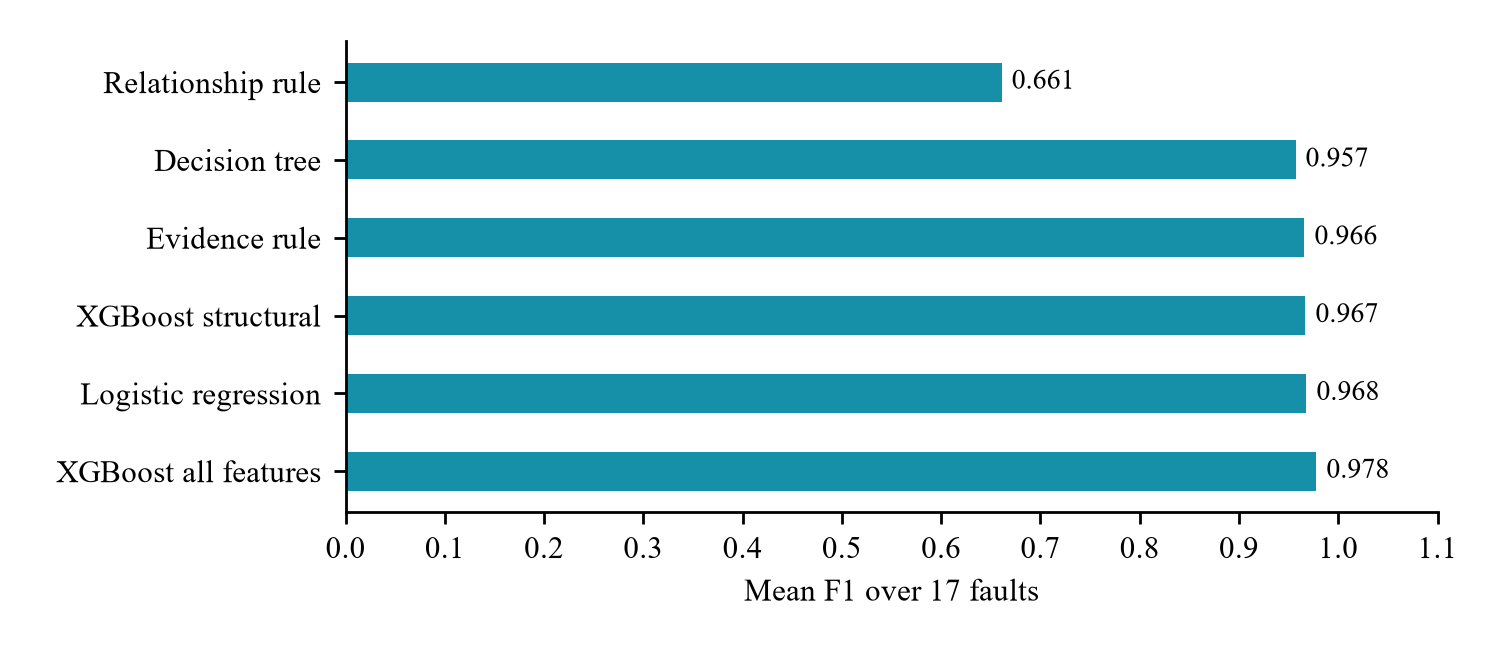
\includegraphics[width=\linewidth]{fig9_1.png}
\end{column}
\end{columns}
\vfill
\begin{simplebox}The value is in the evidence, not the fancy model – XGBoost is no better than simple logistic regression.\end{simplebox}
\end{frame}
\begin{frame}{Result 3: Properties, Leaks and Comparison}
\begin{itemize}
\item \textbf{P1–P4 hold} with protection on (Hypothesis, 120 examples each); P1–P3 fail with it off – proving the tests work.
\item \textbf{4 hidden leak channels found and closed} (error messages, interfaces, counts, refused deletes).
\item \textbf{Timing side channel closed:} 0.352 ms gap before fix $\rightarrow$ no measurable gap after.
\item \textbf{vs. graphql-shield} (13 attacks, 5 normal requests):
\end{itemize}
\begin{center}
\small
\renewcommand{\arraystretch}{1.12}
\begin{tabular}{>{\raggedright\arraybackslash}p{0.287\linewidth}>{\raggedright\arraybackslash}p{0.287\linewidth}>{\raggedright\arraybackslash}p{0.287\linewidth}}
\toprule
\textbf{Measure} & \textbf{GraphQL-Shield} & \textbf{graphql-shield} \\
\midrule
Attacks leaked & 0 / 13 & 0 / 13 \\
\rowcolor{rowgrey}Legitimate requests broken & \textbf{0 / 5} & \textbf{1 / 5} \\
Configuration written & \textasciitilde{}4 entries + owner lookup & 8 entries + 4 rules \\
\bottomrule
\end{tabular}
\end{center}
\end{frame}
\begin{frame}{Result 4: Speed and Self-Repair}
\begin{columns}[c]
\begin{column}{0.52\textwidth}
\begin{itemize}
\item Protection costs \textbf{about 1 ms} per request (with connection pooling).
\item \textbf{Self-repair:} 10 planted config mistakes $\times$ 3 runs:
\begin{itemize}
\item \textbf{30 / 30} detected and fixed by the first verified repair
\item \textbf{33 / 33} wrong repairs refused
\item \textbf{0} legitimate requests blocked
\end{itemize}
\item \textbf{Limitations:} apps and attacks written by us; synthetic ML data; owner-or-admin policies only.
\end{itemize}
\end{column}
\begin{column}{0.46\textwidth}
\centering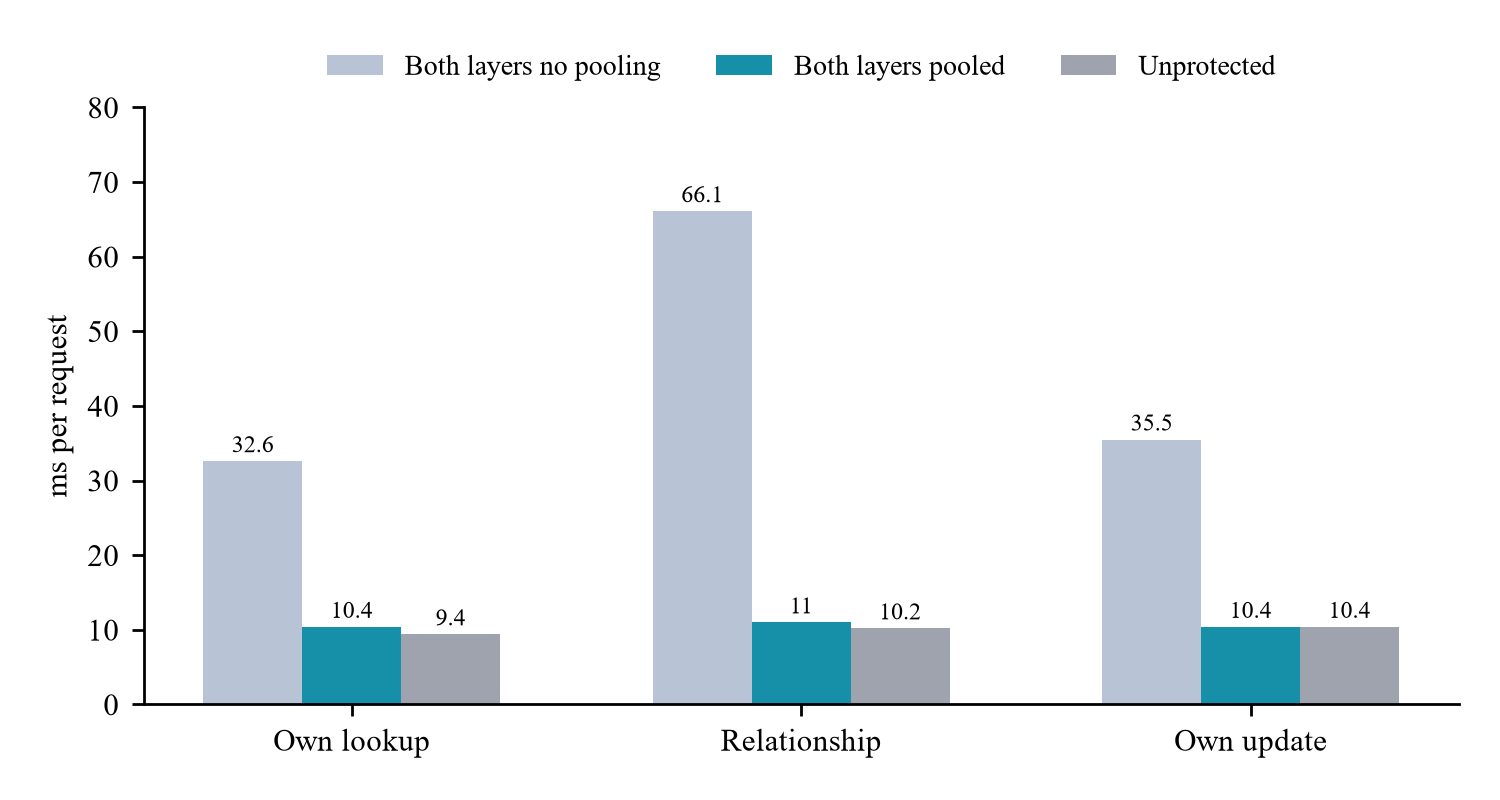
\includegraphics[width=\linewidth]{fig9_2.png}
\end{column}
\end{columns}
\end{frame}

%% ============================================================
\section{Conclusion}
\begin{frame}{Conclusion}
\begin{itemize}
\item Checking ownership at \textbf{two independent points} stops BOLA in every form tested – including hidden relationship attacks.
\item Layer 2’s record of what Layer 1 missed \textbf{detected all 17 planted bugs} with no false alarms.
\item The same evidence \textbf{repaired all 10 configuration mistakes} and refused all 33 wrong fixes.
\item Side channels closed; own data never lost; \textbf{\textasciitilde{}1 ms overhead}; works on 4 Python GraphQL frameworks.
\item Demonstrates defence in depth, complete mediation and fail-safe defaults on a modern API.
\end{itemize}
\vfill
\begin{simplebox}We built a lock that not only keeps intruders out, but also notices when it is weak and fixes itself – with an admin’s approval.\end{simplebox}
\end{frame}

%% ============================================================
\section{Future Scope}
\begin{frame}{Future Scope}
\begin{itemize}
\item Test on real open-source GraphQL apps (e.g. Saleor) with independent attackers.
\item Richer policies: sharing, teams, attribute-based access control.
\item Suggest code patches, not only configuration fixes.
\item Measure timing over real networks; production deployment with TLS, Redis, Kong / Envoy.
\item Train ML models on real anonymised traffic.
\item Port to Node.js (Apollo), Java and Go; add MFA / OAuth 2.0; stream logs to SIEM tools.
\end{itemize}
\end{frame}

\section{References}
\begin{frame}{References (1/2)}
\scriptsize
\begin{enumerate}\setlength{\itemsep}{1pt}
\item[{[1]}] OWASP, “API Security Top 10 – 2023: API1 Broken Object Level Authorization,” 2023.
\item[{[2]}] O. Tsai et al., “GraphQLer: Enhancing GraphQL security with context-aware API testing,” arXiv:2504.13358, 2025.
\item[{[3]}] J. Barach, “AuthProbe: Specification-driven, multi-identity detection of BOLA,” arXiv:2607.20574, 2026.
\item[{[4]}] A. Santos Filho, R. J. Rodríguez, E. L. Feitosa, “Automated BOLA attack detection in REST APIs through OpenAPI to colored Petri nets,” Int. J. Inf. Security, 24(2), 2025.
\item[{[5]}] A. Wu et al., “Rethinking broken object level authorization attacks under zero trust principle,” ACM TOSEM, 2026.
\item[{[6]}] L. Lambers et al., “Taint analysis for graph APIs focusing on broken access control,” LMCS, 22(1), 2026.
\item[{[7]}] graphql-shield, npm package v7.6.5.
\item[{[8]}] O. Hartig, J. Pérez, “Semantics and complexity of GraphQL,” WWW, 2018.
\item[{[9]}] A. Cha et al., “A principled approach to GraphQL query cost analysis,” ESEC/FSE, 2020.
\item[{[10]}] E. Wittern et al., “An empirical study of GraphQL schemas,” ICSOC, 2019.
\item[{[11]}] B. Kaur, “Broken object level authorization in the wild,” arXiv:2605.25865, 2026.
\item[{[12]}] CVE-2022-39275: Saleor mutations did not validate object ID types, 2022.
\end{enumerate}
\end{frame}
\begin{frame}{References (2/2)}
\scriptsize
\begin{enumerate}\setlength{\itemsep}{1pt}\setcounter{enumi}{12}
\item[{[13]}] GraphQL Foundation, “GraphQL specification: Handling field errors.”
\item[{[14]}] J. P. Anderson, “Computer security technology planning study,” ESD-TR-73-51, 1972.
\item[{[15]}] J. H. Saltzer, M. D. Schroeder, “The protection of information in computer systems,” Proc. IEEE, 1975.
\item[{[16]}] J. A. Goguen, J. Meseguer, “Security policies and security models,” IEEE S\&P, 1982.
\item[{[17]}] W. M. McKeeman, “Differential testing for software,” Digital Tech. J., 1998.
\item[{[18]}] Y. Jia, M. Harman, “An analysis and survey of mutation testing,” IEEE TSE, 2011.
\item[{[19]}] K. Claessen, J. Hughes, “QuickCheck,” ICFP, 2000.
\item[{[20]}] D. R. MacIver et al., “Hypothesis: A new approach to property-based testing,” JOSS, 2019.
\item[{[21]}] A. Ratner et al., “Snorkel: Rapid training data creation with weak supervision,” PVLDB, 2017.
\item[{[22]}] T. Chen, C. Guestrin, “XGBoost: A scalable tree boosting system,” KDD, 2016.
\item[{[23]}] S. M. Lundberg, S.-I. Lee, “A unified approach to interpreting model predictions,” NeurIPS, 2017.
\end{enumerate}
\end{frame}

\section{Research Paper Template}
\begin{frame}{Research Paper (IEEE Conference Template)}
\begin{center}
\small
\renewcommand{\arraystretch}{1.12}
\begin{tabular}{>{\raggedright\arraybackslash}p{0.160\linewidth}>{\raggedright\arraybackslash}p{0.738\linewidth}}
\toprule
\textbf{Item} & \textbf{Details} \\
\midrule
Title & GraphQL-Shield: Dual-Layer Enforcement Against GraphQL BOLA with Cross-Layer Coverage Evidence \\
\rowcolor{rowgrey}Template & IEEE Conference (two-column) \\
Authors & [Author 1], [Author 2], [Author 3], [Author 4] \\
\rowcolor{rowgrey}Keywords & GraphQL, API security, BOLA, access control, defense in depth, fault injection, property-based testing \\
Length & 8 pages, 23 references, 2 figures, 7 tables \\
\rowcolor{rowgrey}Files & paper/main.tex, paper/references.bib, paper/main.pdf \\
\bottomrule
\end{tabular}
\end{center}
\begin{simplebox}The full work is written up as an 8-page IEEE two-column research paper, compiled from LaTeX.\end{simplebox}
\end{frame}

\begin{frame}
  \centering
  \vfill
  {\Huge\textbf{\color{navy}Thank You}}\\[12pt]
  {\Large Questions?}\\[18pt]
  \small Code: \url{https://github.com/Chinmayanand03/GraphQL-Shield-}
  \vfill
\end{frame}

\end{document}
